% !TeX root = ../main.tex
\chapter{Introduction and outline}
\label{chap:introduction}
\section{Quantum chromodynamics and its phase diagram}
\begin{figure}[h]
    \centering 
    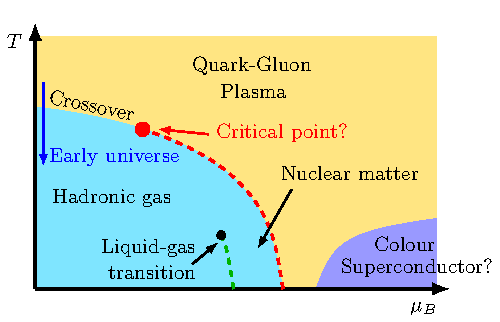
\includegraphics[scale=1.3]{figures/phase_diagram.pdf}
    \caption[The phase diagram of QCD]{Conjectured phase diagram of Quantum Chromodynamics. At low temperature and chemical potential, Quantum Chromodynamics exists in a chirally broken state, where quarks and gluons are confined into hadrons and cannot be observed as single particles. As temperature or chemical potential are raised above a critical treshold, chiral symmetry is restored and particles lie in a quark-gluon plasma state. The existence and location of the critical point, as well as the colour superconducting state, is still matter of ongoing research.}
    \label{fig:QCD_phase_diagram}
\end{figure}
\noindent Quantum Chromodynamics (QCD) plays a fundamental role in our understanding of the Standard Model. It is the theory describing the strong force among quarks, gluons and the composition of hadrons such as protons and neutrons, which constitutes the base of most of the matter around us. \\
The diagram reported in Figure \ref{fig:QCD_phase_diagram} illustrate the phases of QCD as a function of temperature $T$ and baryon chemical potential $\mu_B$.
At low temperature and chemical potential, QCD exhibits confinement \cite{confinement_wilson,Greensite:2011zz}, a phenomenon for which only colour-neutral states can be observed. The confined phase is characterised by a spontaneously broken chiral symmetry. The restoration of chiral symmetry is expected in the transition towards a quark-gluon plasma at high temperatures (roughly $T > 160~\text{MeV}$) or chemical potential (roughly $\mu_B > 1~\text{GeV}$) \cite{Masayuki1989,Stephanov_1998,Berges_1999,doi:10.1142/S0217751X92001757,Endroedi_2014}. Moreover, also new states of matter are hypothesized, such as the existence of the colour superconducting state \cite{colorsuper1,colorsuper2,colorsuper3}. \\
Much more has to be studied in the phase diagram, such as the precise determination of the location and nature of the critical point (if it exists at all). It is a huge challenge that needs a combination of theory, experiments, and simulations. \\
On the theoretical side, a wide number of results have been obtained from functional methods such as the functional renormalisation group (fRG) and Dyson-Schwinger equations (DSE) \cite{QCDphase,QCDphase2,Gao_2021}.
The major experiments are performed at the Relativistic Heavy Ion Collider (RHIC) in New York and the Large Hadron
Collider (LHC) at CERN. The Facility for Antiproton and Ion Research (FAIR) in Darmstadt, Germany, is a new collider under construction. On the simulation side, lattice field theory has become the standard approach to study QCD and particle physics and a large number of results have been obtained \cite{wuppertal,201915,Endroedi_2014,sym13112079}. \\
For a more detailed overview of the features of the QCD phase diagram see refs. \cite{phasediag1,Bellwied2015}.
\section{Lattice Field Theory}
Computing physical quantities from first principle approaches is not only hard to do, but often results impossible since a na\"ive approach yields diverging results. In fact, most quantum field theories need to be regularised by introducing an ultraviolet cutoff. To do this, one often relies on expansion techniques such as perturbation theory, in which one tries to regularise the theory order by order in an expansion on the interaction coupling, yielding finite quantities that depend on the truncation order.  While this method is capable of producing incredibly precise results, it fails completely in treating non-perturbative phenomena, namely effects that cannot be captured by any order in the expansion or that are typical of strongly interacting systems.
Phenomena such as confinement are non-perturbative.\\
A standard formulation of quantum field theory is also not very suitable for numerical computations since the path integral measure and the action are infinite dimensional objects. \\
Lattice field theory \cite{Montvay1994QuantumLattice,rothe_LGT,gattringer_LQCD,creutz_2023}, which was proposed by Kenneth G. Wilson in 1974 \cite{wilson_lqcd}, is meant at first as a powerful non-perturbative regularisation tool to prevent divergences to occur and render the computation of the correlation functions finite. Moreover, it also provides a framework to study quantum field theory numerically on a computer. In order to accomplish this, one defines the theory on a spacetime lattice and makes use of statistical methods such as Monte Carlo algorithms to compute observables. 
One should not view the lattice as an approximation to the continuum theory. It rather defines a theory that is undefined directly in the continuum \cite{Wiese:2009qsa}. One may then wonder how to reconstruct a result in the continuum theory, keeping it finite, and matching it to the physically measured one. This task, far from being simple, will be  discussed in the next chapters.\\
Lattice QCD does not come without problems. Simulations at large chemical potential are in fact hard due to the presence of the sign problem. Amongst other candidates, a promising method aimed at solving the issue is Stochastic Quantisation based on the Complex Langevin equation \cite{Gert_Aarts_2008,Berger_2021,Seiler_2018_status,Aarts_2010}. In fact, it successfully produced a wide number of results in studying the phase diagram of QCD and similar theories \cite{attanasio,Attanasio_2020,langelage2013onset,sinclair2016complex,Sexty_2014}. For a review of the method, we refer to \cite{Aarts_2016,Aarts_2013}. Here, we just want to mention that convergence of the Complex Langevin algorithm often requires gauge cooling techniques \cite{gaugecool} that remove configurations with large ultraviolet fluctuations. 
In this sense, the cooling technique that will be presented in this work could be of great benefit to the algorithm.

\section{The emergence of effective theories}
A central role in our investigation will be played by the Wilsonian perspective of the Renormalisation Group (RG) \cite{WilsonRG1,WilsonRG2,WILSON197475}. Within this paradigm, renormalisation ceases to be merely a tool for taming divergences; 
the Wilsonian RG approach provides a rigorous way to perform a change of scale in a physical theory. The Wilson framework naturally brings to the concept of effective theory, a model where irrelevant degrees of freedom are averaged out and replaced by an effective description in terms of the relevant quantities at the given scale.  \\
Effective theories are widely used to study QCD, aiming at tailoring to specific aspects of the strong force dynamics. 
Among others, we mention the Nambu\textendash{}Jona-Lasinio model \cite{Nambu1961DynamicalI, Nambu1961DynamicalII}, the Gross\textendash{}Neveu model \cite{grossneveu}, and the Quark-Meson model \cite{quarkmeson1,quarkmeson2,quarkmeson3}. All of these theories are Yukawa-type theories, namely theories that can be described in terms of a fermion-boson-fermion interaction. This fact motivates the choice of the model in our work.

\section{Outline}
Chapter \ref{chap:background} is devoted to the introduction of the theoretical background that supports this work.
We will start with the Kadanoff and Wilson approach to renormalisation in statistical physics and quantum field theory.
Lattice field theory is then introduced as a powerful tool to simulate quantum field theory numerically and the basics of the formulation are provided.     
We then turn to stochastic quantisation, the relation between noise and quantum fluctuations, and how the standard formulation is modified by the presence of coloured noise. 
This results in a deep connection between coloured stochastic quantisation and the renormalisation group. We then turn to the discussion of chiral symmetry and its breaking, both in the continuum and on the lattice.
The chapter ends with a description of the model on which the above techniques are applied, namely a Yukawa theory. \\~\\
Chapter \ref{chapt:methods} is devoted to detail techniques and methodologies of the project.
We will start by explaining how the continuum model is discretised on a spacetime lattice and how it can be simulated via a Monte Carlo method based on stochastic quantisation.
Some possible applications of coloured noise in lattice QFT are then listed, and the numerical experiments that are carried out in the last chapter are described.
The chapter ends with a description of the relevant observables that are employed to study a lattice quantum field theory. \\~\\
Chapters \ref{chapt:results_preliminary} and \ref{chapt:results_coloured} are devoted to the numerical investigation.
First, a preliminary analysis is carried out. The procedure of extracting fermionic masses in the simulation is illustrated, and a panoramic view over the general phase structure of the theory is provided. The latter will guide the choice of parameter settings for all the simulations.
It is then shown how coloured noise can be used to provide a smooth interpolation between the fully classical and fully quantum pictures.
The introduction of noise can cause a qualitative change in the behaviour of the system. In particular, it is shown how it can trigger a phase transition in the model.
Finally, the connection with the Kadanoff-Wilson RG is exploited to cool a simulation by systematically encoding ultraviolet (UV) fluctuations in a redefinition of the classical action, without altering the physical content of the theory.